\documentclass[10pt,a4paper]{article}
\usepackage[margin=2.0cm]{geometry}
\usepackage[T1]{fontenc}
\usepackage[utf8]{inputenc}
\usepackage{lmodern}
\usepackage{microtype}
\usepackage{amsmath,amssymb,amsthm,mathtools,bm}
\usepackage{booktabs,tabularx,array,multirow,longtable}
\usepackage{enumitem}
\usepackage{xcolor}
\usepackage{graphicx}
\usepackage{tikz}
\usetikzlibrary{arrows.meta,positioning,fit,calc,shapes.geometric,backgrounds}
\usepackage[most]{tcolorbox}
\usepackage{url}
\usepackage{hyperref}
\usepackage[nameinlink,capitalise]{cleveref}
\usepackage[numbers,sort&compress]{natbib}
\usepackage{fancyhdr}
\usepackage{lastpage}
\usepackage{caption}
\usepackage{subcaption}
\usepackage{float}
\usepackage{listings}

\definecolor{mmalsgreen}{HTML}{315D47}
\definecolor{mmalsgold}{HTML}{A17C28}
\definecolor{mmalsblue}{HTML}{2E5C88}
\definecolor{mmalsred}{HTML}{8A3A32}
\definecolor{lightgreen}{HTML}{EFF6F1}
\definecolor{lightblue}{HTML}{EEF4F9}
\definecolor{lightgold}{HTML}{FBF7EC}
\definecolor{lightred}{HTML}{FAF0EF}

\hypersetup{
  colorlinks=true,
  linkcolor=mmalsblue,
  citecolor=mmalsgreen,
  urlcolor=mmalsred,
  pdftitle={From Functional Route Memory to Learnable Geometry},
  pdfauthor={Guillaume Harbonnier},
  pdfsubject={Riemannian architecture and experimental roadmap for MMALS}
}

\pagestyle{fancy}
\fancyhf{}
\lhead{MMALS Riemannian Learning Architecture}
\rhead{Research article v1.0}
\cfoot{\thepage/\pageref{LastPage}}
\setlength{\headheight}{14pt}

\newtheorem{definition}{Definition}
\newtheorem{proposition}{Proposition}
\newtheorem{hypothesis}{Hypothesis}
\newtheorem{remark}{Remark}
\newtheorem{gate}{Evidence gate}

\newcommand{\MMALS}{\textsc{MMALS}}
\newcommand{\RGM}{\textsc{RGM}}
\newcommand{\SPD}{\mathbb{S}_{++}}
\newcommand{\simplex}{\Delta}
\newcommand{\cM}{\mathcal{M}}
\newcommand{\cL}{\mathcal{L}}
\newcommand{\cD}{\mathcal{D}}
\newcommand{\cT}{\mathcal{T}}
\newcommand{\cC}{\mathcal{C}}
\newcommand{\R}{\mathbb{R}}
\newcommand{\E}{\mathbb{E}}
\newcommand{\Tr}{\operatorname{Tr}}
\newcommand{\diag}{\operatorname{diag}}
\newcommand{\Exp}{\operatorname{Exp}}
\newcommand{\Log}{\operatorname{Log}}
\newcommand{\PT}{\operatorname{PT}}
\newcommand{\softmax}{\operatorname{softmax}}
\newcommand{\KL}{\operatorname{KL}}

\newtcolorbox{statusbox}{colback=lightgold,colframe=mmalsgold,title=Scientific status,fonttitle=\bfseries}
\newtcolorbox{engineeringbox}{colback=lightgreen,colframe=mmalsgreen,title=Engineering interpretation,fonttitle=\bfseries}
\newtcolorbox{warningbox}{colback=lightred,colframe=mmalsred,title=Non-claim and falsification boundary,fonttitle=\bfseries}
\newtcolorbox{sourcebox}{colback=lightblue,colframe=mmalsblue,title=Source tier note,fonttitle=\bfseries}

\title{\textbf{From Functional Route Memory to Learnable Geometry}\\[0.4em]
\large A Riemannian Architecture, Evidence Discipline, and Experimental Roadmap for Mycelium-Inspired Mutualistic Adaptive Learning Systems}
\author{Guillaume Harbonnier\\MMALS Research Program\\\small \url{https://github.com/gharbonnier78/geometry-mmalls-g1}}
\date{28 July 2026 -- Research article and implementation specification v1.0}

\begin{document}
\maketitle

\begin{statusbox}
This article is a research integration and experimental specification. It does not claim that \MMALS{} has already demonstrated a general continual-learning advantage, that a learned Riemannian metric is necessarily superior to a fixed metric, or that biological mycelium and mathematical manifolds are equivalent mechanisms. It translates established Riemannian deep-learning components into falsifiable \MMALS{} hypotheses and preserves negative internal evidence that geometric regularization can over-constrain plasticity.
\end{statusbox}

\begin{abstract}
Mycelium-Inspired Mutualistic Adaptive Learning Systems (\MMALS{}) treat continual learning as adaptive cooperation among specialist hosts mediated by a routing and transformation substrate. Early prototypes established a crucial distinction: preserving a routing vector is not equivalent to preserving the function computed through that route. Later experiments therefore introduced functional route memory, latent distillation, and diagnostics for route, output, transformation, and Jacobian drift. Yet most of these quantities remain measured with fixed Euclidean norms, even when the objects being compared are probability distributions, covariance-like descriptors, correlation matrices, or structured transformation states.

This article develops a conservative Riemannian extension of the \MMALS{} program using the reusable modules, manifold-specific networks, and learnable geometries synthesized in Ziheng Chen's 2026 doctoral thesis on Riemannian deep learning. The proposal has five parts. First, route distributions are treated intrinsically on the probability simplex using Fisher-Rao geometry rather than raw coefficient error. Second, functional memory is represented by symmetric positive-definite or full-rank correlation descriptors whose drift is measured by fixed or learnable pullback metrics. Third, intrinsic normalization and classification are introduced only where their manifold assumptions are satisfied, using Lie-group or gyrogroup normalization and Riemannian multinomial logistic regression. Fourth, the geometry is allowed to adapt through a constrained family of pullback maps, with Cholesky product geometries retained as a fast and numerically stable control. Fifth, context, route, host function, memory, and output are modeled as a coupled product geometry, but every added component must beat simpler null models under matched compute and memory budgets.

The article contributes a complete mathematical specification, an architecture diagram, hypotheses, ablations, source tiers, claim gates, failure criteria, and a staged experiment protocol aligned with the existing Geometry-\MMALS{} G1 repository. The central research claim is deliberately narrow: a geometry is useful only if its intrinsic distances and transport operators predict functional forgetting better than Euclidean diagnostics, and if geometry-aware learning improves retention, plasticity, calibration, or cost without hiding degradation elsewhere.
\end{abstract}

\noindent\textbf{Keywords:} continual learning; geometric deep learning; Riemannian manifolds; functional memory; adaptive routing; SPD matrices; information geometry; metric learning; mixture of experts; evidence governance.

\tableofcontents
\newpage


\section{Motivation and research question}

\subsection{The problem after functional route memory}
The minimal \MMALS{} computation has specialist hosts $g_i$, host-specific fungal transformations $T_i$, an input- and context-conditioned route $r$, and a synthesized latent state
\begin{align}
  z_i(x) &= g_i(x), \\
  \tilde z_i(x) &= T_i(z_i(x)), \\
  r_i(x,c) &= \frac{\exp(a_i(x,c)/\tau)}{\sum_j \exp(a_j(x,c)/\tau)}, \\
  z_f(x,c) &= \sum_{i=1}^{H} r_i(x,c)\tilde z_i(x), \\
  \hat y &= h(z_f).
  \label{eq:mmals-basic}
\end{align}
The v0.7--v0.9 line showed why route memory alone is insufficient: $r$ may remain stable while the host representation, the transformation $T_i$, or the synthesized function changes. In the reported v0.9 diagnostic, route-memory-only controlled route drift but allowed substantial latent drift, whereas latent-preserving variants strongly reduced the functional drift. The appropriate memory object is therefore not merely a path identifier, but the mediated function computed through the path \citep{harbonnier2026v09,harbonnier2026v08}.

The next problem is more subtle. Even after accepting functional memory, the project still uses fixed distances for heterogeneous objects:
\begin{itemize}[leftmargin=1.5em]
  \item Euclidean mean-square error for route vectors constrained to a simplex;
  \item Euclidean error for latent states whose covariance and local sensitivity may matter more than coordinates;
  \item Frobenius norms for transformations with non-trivial spectral structure;
  \item independent scalar penalties for co-evolving route, latent, output, and Jacobian states.
\end{itemize}
A lower Euclidean distance does not automatically mean a smaller functional change. Conversely, a coordinate change may be harmless if it follows an invariant direction of the model. The research question is therefore:

\begin{quote}
Can \MMALS{} learn or select a geometry in which route and functional-memory distances are better aligned with forgetting, transfer, uncertainty, and computational cost than fixed Euclidean diagnostics, without creating geometric rigidity?
\end{quote}

\subsection{Why the 2026 Riemannian deep-learning thesis is relevant}
Chen's thesis develops Riemannian deep learning at three levels: reusable modules across manifolds, manifold-specific neural networks, and the design of the underlying geometry itself \citep{chen2026thesis}. Its most relevant contributions for \MMALS{} are:
\begin{enumerate}[leftmargin=1.7em]
  \item \textbf{Intrinsic normalization.} Lie Group Batch Normalization controls Riemannian sample mean and variance using group translations and tangent-space scaling. Gyrogroup Batch Normalization extends the principle beyond Lie groups to a wider class of manifolds.
  \item \textbf{Intrinsic classification.} Riemannian multinomial logistic regression replaces Euclidean tangent-space classification with a formulation that uses the manifold logarithm and Riemannian trigonometry.
  \item \textbf{Structured networks.} Hyperbolic Proper Velocity networks offer an unconstrained representation intended to reduce boundary instability; full-rank correlation networks operate directly on normalized dependence structure.
  \item \textbf{Learnable metrics.} Adaptive Log-Euclidean Metrics construct a family of pullback geometries through parameterized matrix logarithms, retaining closed-form Riemannian operators and modest extra computation.
  \item \textbf{Fast stable controls.} Product Cholesky geometries yield closed-form operators while avoiding repeated scalar logarithm and exponential operations that can become unstable.
\end{enumerate}

The thesis does not study continual learning, \MMALS{}, task-free context inference, or mycelium-inspired mutualism. Its role is therefore not empirical validation of \MMALS{}, but a mature mathematical and software design library from which testable components can be selected.

\begin{sourcebox}
The source hierarchy is explicit. Peer-reviewed component papers underlying the thesis are Tier 1. The doctoral thesis is Tier 2 as an integrated primary synthesis. Executed \MMALS{} runs are Tier 3 project evidence. The architecture and hypotheses proposed in this article are Tier 4 until independently tested. The complete machine-readable mapping is supplied in \texttt{governance/source\_tiers.yaml} and \texttt{governance/claim\_manifest.yaml}.
\end{sourcebox}


\section{Current MMALS evidence and constraints}

\subsection{What the existing prototypes support}
The existing evidence should be carried forward rather than reset by a new geometric vocabulary.

\paragraph{Functional memory is more meaningful than route identity.}
The v0.8 evidence harness reported a full-functional-memory variant with final average accuracy approximately $0.9914$ and average forgetting approximately $4.4\times 10^{-4}$ in its controlled task-incremental FashionMNIST setting, while the v0.9 diagnostic showed that route drift and functional latent drift explain different failure modes \citep{harbonnier2026v08,harbonnier2026v09}. These are internal controlled results, not general continual-learning claims.

\paragraph{Geometry regularization can harm plasticity.}
The v0.12--v0.13.1 co-evolution branch investigated transformation, spectral, and Jacobian preservation. In the v0.13.1 smoke run, output distillation remained the best method: final average accuracy was $0.904$ with forgetting $0.0263$, while warm weak adaptive co-evolution reached $0.872$ with forgetting $0.0825$. Hard frozen transformations were worse still \citep{harbonnier2026v12,harbonnier2026v131}. This negative result is central: lower geometric drift is not a success when the model learns new contexts less effectively.

\paragraph{Grounded context geometry is currently stronger than route geometry.}
The Geometry-\MMALS{} G1 repository reports replicated evidence that covariance-aware context geometry improves stress and held-out context decoding on a controlled rotation factor, while route geometry, host specialization, memory transport, and operational superiority remain unqualified \citep{geometrymmalsg1}. This suggests that the first Riemannian intervention should target diagnostics and context/functional descriptors, not an immediate replacement of the whole router.

\subsection{Design constraints inherited by the new article}
The proposed architecture adopts the existing G1 simplicity axiom: exotic geometry is introduced only after a simpler Euclidean, simplex, or fixed-metric null model fails. The following constraints are mandatory:
\begin{enumerate}[leftmargin=1.7em]
  \item no explicit task identifier at inference in the mature protocol;
  \item matched trainable parameters, active compute, replay memory, and optimization budget;
  \item joint reporting of retention and intransigence/plasticity;
  \item raw per-seed metrics and failed runs preserved;
  \item metric selection frozen before qualification data are evaluated;
  \item no claim based only on a two-dimensional visualization;
  \item no use of geometry as a synonym for any latent representation.
\end{enumerate}


\section{Riemannian design principles for MMALS}

\subsection{Geometry must match the object}
A Riemannian metric assigns an inner product to each tangent space. It determines distances, geodesics, logarithmic and exponential maps, parallel transport, means, variances, and optimization updates. Changing the metric can therefore alter not only interpretation but parameterization, numerical stability, and computation \citep{absil2008,amari2016,chen2026thesis}.

For \MMALS{}, no single manifold should be imposed on all layers. The proposed state is a product of objects with distinct geometries:
\begin{equation}
  \cM_{\MMALS}
  = \cM_c \times \cM_r \times \cM_f \times \cM_T \times \cM_m \times \cM_y,
  \label{eq:product-manifold}
\end{equation}
where $\cM_c$ is inferred context, $\cM_r$ routing, $\cM_f$ functional state, $\cM_T$ transformation geometry, $\cM_m$ memory, and $\cM_y$ output distributions. A product metric may be written
\begin{equation}
  g_{\bm{\lambda}}
  = \lambda_c g_c \oplus \lambda_r g_r \oplus \lambda_f g_f
    \oplus \lambda_T g_T \oplus \lambda_m g_m \oplus \lambda_y g_y,
  \label{eq:product-metric}
\end{equation}
with coefficients selected on development data and frozen for qualification. The product is a bookkeeping discipline, not evidence that every component is curved.

\subsection{Route geometry on the probability simplex}
The router output lies in the open simplex
\begin{equation}
  \simplex^{H-1}_{\circ}
  = \left\{r\in\R^H: r_i>0,\ \sum_i r_i=1\right\}.
\end{equation}
A raw Euclidean route penalty
\begin{equation}
  \cL_{r,2}=\|r-r^\star\|_2^2
\end{equation}
ignores the statistical meaning of $r$. Under Fisher-Rao geometry, the square-root map embeds the simplex into the positive orthant of a sphere. A closed-form distance is
\begin{equation}
  d_{\mathrm{FR}}(r,s)
  = 2\arccos\!\left(\sum_{i=1}^{H}\sqrt{r_i s_i}\right).
  \label{eq:fisher-rao}
\end{equation}
The intrinsic route-memory loss becomes
\begin{equation}
  \cL_{r,\mathrm{FR}}
  = \E_{x\sim\cD_{\mathrm{mem}}}
    \left[d_{\mathrm{FR}}\big(r_{\theta}(x),r_{\theta^\star}(x)\big)^2\right].
  \label{eq:route-loss}
\end{equation}
This loss is not assumed superior. It is tested against Euclidean, Jensen-Shannon, Hellinger, and no-route-memory controls.

\begin{engineeringbox}
Two routes can have the same Euclidean gap yet different statistical meaning near the boundary. Moving probability mass away from a nearly impossible host may be more consequential than the same coordinate shift in the interior. Fisher-Rao geometry supplies a principled null hypothesis for that distinction.
\end{engineeringbox}

\subsection{Functional memory as an SPD descriptor}
The synthesized vector $z_f$ is only one sample-level view of a route-function. A memory descriptor can preserve local second-order structure. For a context or memory cell $k$, define
\begin{equation}
  C_k
  = \frac{1}{B-1}\sum_{b=1}^{B}
    (u_b-\bar u)(u_b-\bar u)^\top + \epsilon I,
  \qquad C_k\in\SPD^{d},
  \label{eq:spd-memory}
\end{equation}
where $u_b$ may concatenate selected host outputs, the synthesized latent state, and low-rank Jacobian probes. The regularization $\epsilon I$ ensures positive definiteness.

A fixed Log-Euclidean distance is
\begin{equation}
  d_{\mathrm{LE}}(C_1,C_2)
  = \|\log C_1-\log C_2\|_F.
  \label{eq:le-distance}
\end{equation}
This supplies a stronger descriptor than pointwise MSE when forgetting is associated with changes in covariance, anisotropy, or cross-host dependence.

An alternative full-rank correlation descriptor removes marginal scale:
\begin{equation}
  R_k = D_k^{-1/2} C_k D_k^{-1/2},
  \qquad D_k=\diag(C_k),
  \label{eq:corr-memory}
\end{equation}
allowing the experiment to separate ``the function changed scale'' from ``the dependence structure changed.'' Chen's correlation networks are relevant because they construct layers and backpropagation directly on this manifold rather than treating correlation matrices as unconstrained Euclidean arrays \citep{chen2026cornet,chen2026thesis}.

\subsection{Learnable pullback geometry}
A pullback metric transfers Euclidean geometry through a diffeomorphism $\phi_\eta:\SPD^d\rightarrow\mathbb{S}^d$. Define
\begin{equation}
  g^{\eta}=\phi_\eta^* g_E,
  \qquad
  d_{\eta}(C_1,C_2)
  = \|\phi_\eta(C_1)-\phi_\eta(C_2)\|_F.
  \label{eq:pullback}
\end{equation}
The associated operators inherit closed forms:
\begin{align}
  \Exp^{\eta}_{C}(V)
  &= \phi_\eta^{-1}\big(\phi_\eta(C)+(\phi_\eta)_{*,C}V\big),\\
  \Log^{\eta}_{C_1}(C_2)
  &= (\phi_\eta^{-1})_{*,\phi_\eta(C_1)}
     \big(\phi_\eta(C_2)-\phi_\eta(C_1)\big),\\
  \PT^{\eta}_{C_1\to C_2}(V)
  &= (\phi_\eta^{-1})_{*,\phi_\eta(C_2)}
     \circ (\phi_\eta)_{*,C_1}(V).
  \label{eq:pullback-ops}
\end{align}
Adaptive Log-Euclidean Metrics instantiate this idea with parameterized matrix logarithms and retain an abelian Lie-group structure \citep{chen2024alem,chen2026thesis}. For \MMALS{}, a conservative implementation uses a monotone spectral map
\begin{equation}
  \phi_\eta(C)
  = U\diag\big(f_{\eta,1}(\lambda_1),\ldots,f_{\eta,d}(\lambda_d)\big)U^\top,
  \label{eq:spectral-map}
\end{equation}
where $C=U\diag(\lambda)U^\top$ and each $f_{\eta,j}$ is constrained to remain smooth and strictly monotone. The metric parameters are regularized toward the natural logarithm:
\begin{equation}
  \cL_{\mathrm{metric}}
  = \|\eta-\eta_{\log}\|_2^2
  + \gamma_{\mathrm{cond}}\,\Psi_{\mathrm{condition}}(\phi_\eta).
  \label{eq:metric-reg}
\end{equation}
The purpose is not unrestricted metric fitting. It is to learn which spectral directions of functional change matter while retaining invertibility, numerical stability, and a fixed low-dimensional parameter budget.

\subsection{Fast Cholesky geometry as the stability control}
Learnable spectral maps require eigendecomposition and may become sensitive near repeated eigenvalues. Chen's product Cholesky geometries expose the lower-triangular product structure $C=LL^\top$ and construct fast, stable closed-form operators, including Power-Cholesky and Bures-Wasserstein-Cholesky metrics \citep{chen2026cholesky,chen2026thesis}. In the \MMALS{} protocol, a Cholesky metric is not merely another candidate. It is the mandatory efficiency and stability control against which a learnable spectral metric must justify its extra cost.

The comparison records:
\begin{equation}
  \text{utility per active cost}
  = \frac{\Delta\text{retention} - \alpha\Delta\text{intransigence}
  + \beta\Delta\text{calibration}}{
  1+\rho_{\mathrm{time}}+\rho_{\mathrm{memory}}+\rho_{\mathrm{instability}}}.
  \label{eq:utility-cost}
\end{equation}
No single scalar replaces the underlying metrics; it is a secondary summary after all components are reported.


\section{Proposed Riemannian MMALS architecture}

\subsection{Architecture overview}
The proposed Riemannian Geometry for MMALS track, abbreviated \RGM{}, adds intrinsic operators at selected interfaces rather than rebuilding every host.

\begin{figure}[H]
\centering
\resizebox{\textwidth}{!}{%
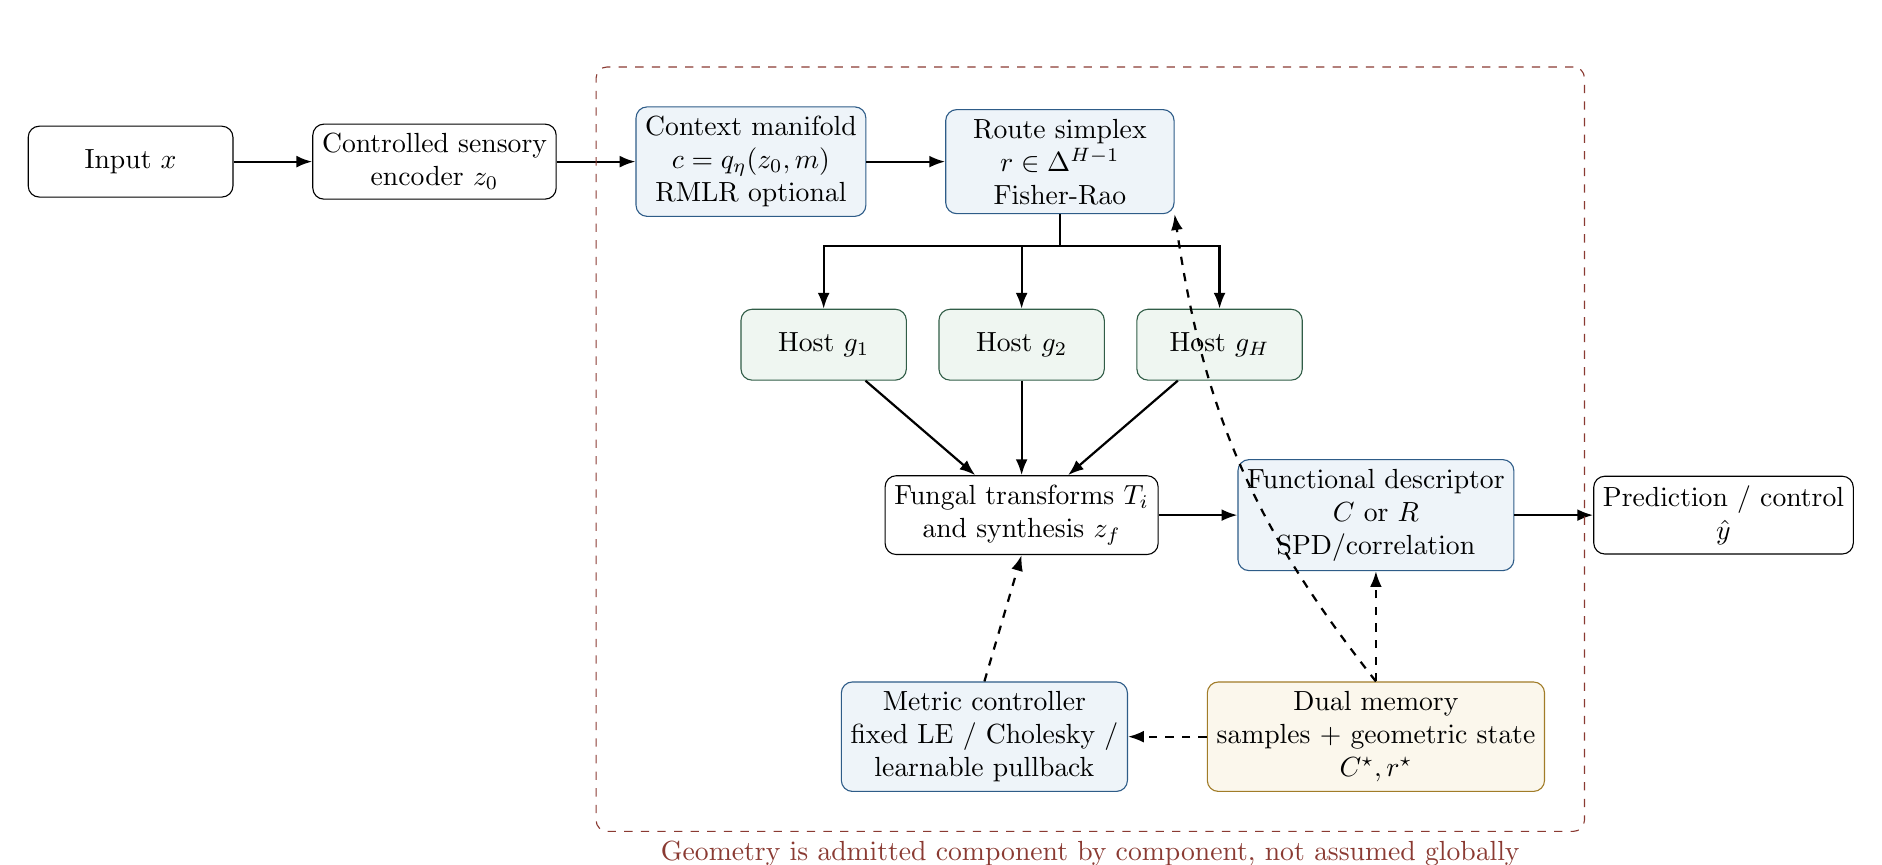
\begin{tikzpicture}[
  node distance=8mm and 10mm,
  block/.style={draw,rounded corners,minimum width=26mm,minimum height=9mm,align=center,fill=white},
  geom/.style={draw,rounded corners,minimum width=29mm,minimum height=10mm,align=center,fill=lightblue,draw=mmalsblue},
  host/.style={draw,rounded corners,minimum width=21mm,minimum height=9mm,align=center,fill=lightgreen,draw=mmalsgreen},
  memory/.style={draw,rounded corners,minimum width=30mm,minimum height=10mm,align=center,fill=lightgold,draw=mmalsgold},
  arrow/.style={-{Latex[length=2mm]},thick},
  dashedarrow/.style={-{Latex[length=2mm]},thick,dashed}
]
  \node[block] (x) {Input $x$};
  \node[block,right=of x] (enc) {Controlled sensory\\encoder $z_0$};
  \node[geom,right=of enc] (context) {Context manifold\\$c=q_\eta(z_0,m)$\\RMLR optional};
  \node[geom,right=of context] (route) {Route simplex\\$r\in\Delta^{H-1}$\\Fisher-Rao};

  \node[host,below=12mm of route,xshift=-30mm] (h1) {Host $g_1$};
  \node[host,right=4mm of h1] (h2) {Host $g_2$};
  \node[host,right=4mm of h2] (h3) {Host $g_H$};
  \node[block,below=12mm of h2] (synth) {Fungal transforms $T_i$\\and synthesis $z_f$};
  \node[geom,right=of synth] (spd) {Functional descriptor\\$C$ or $R$\\SPD/correlation};
  \node[block,right=of spd] (head) {Prediction / control\\$\hat y$};

  \node[memory,below=14mm of spd] (mem) {Dual memory\\samples + geometric state\\$C^\star,r^\star$};
  \node[geom,left=of mem] (metric) {Metric controller\\fixed LE / Cholesky /\\learnable pullback};

  \draw[arrow] (x)--(enc);
  \draw[arrow] (enc)--(context);
  \draw[arrow] (context)--(route);
  \draw[arrow] (route.south) -- ++(0,-4mm) -| (h1.north);
  \draw[arrow] (route.south) -- ++(0,-4mm) -| (h2.north);
  \draw[arrow] (route.south) -- ++(0,-4mm) -| (h3.north);
  \draw[arrow] (h1)--(synth);
  \draw[arrow] (h2)--(synth);
  \draw[arrow] (h3)--(synth);
  \draw[arrow] (synth)--(spd);
  \draw[arrow] (spd)--(head);
  \draw[dashedarrow] (mem)--(spd);
  \draw[dashedarrow] (mem.west)--(metric.east);
  \draw[dashedarrow] (metric.north)--(synth.south);
  \draw[dashedarrow] (mem.north) to[bend left=15] (route.south east);

  \node[draw=mmalsred,dashed,rounded corners,fit=(context)(route)(h1)(h3)(synth)(spd)(metric)(mem),inner sep=5mm,label={[text=mmalsred]below:Geometry is admitted component by component, not assumed globally}] {};
\end{tikzpicture}%
}
\caption{Proposed selective Riemannian extension of \MMALS{}. The sensory encoder and hosts may remain ordinary neural networks. Intrinsic geometry is introduced at the context, route, functional-descriptor, and memory-transport interfaces only when ablations justify it.}
\label{fig:architecture}
\end{figure}

\subsection{Context inference with intrinsic classification}
The mature model infers context without a task identifier. Let $c\in\cM_c$ be a structured context representation and $\mu_k\in\cM_c$ context prototypes. A Euclidean classifier applies a linear map to coordinates. Riemannian MLR instead constructs logits from intrinsic geometry, requiring a logarithmic map and a tangent normal $A_k\in T_{\mu_k}\cM_c$ \citep{chen2024rmlr,chen2026thesis}. A generic score can be written schematically as
\begin{equation}
  \ell_k(c)
  = b_k + \langle A_k,\Log_{\mu_k}(c)\rangle_{\mu_k}
  \cdot \omega_k(c),
  \label{eq:rmlr-context}
\end{equation}
where $\omega_k$ encodes the Riemannian-trigonometric normalization required by the selected formulation. The operational rule is strict: RMLR is tested only after the context representation has a declared manifold and valid logarithmic map. It is not used as decorative terminology for an unconstrained vector.

\subsection{Intrinsic normalization at stable interfaces}
Sequential training can shift the mean and variance of structured states. LieBN and GyroBN offer principled normalization when the state manifold admits the corresponding algebraic structure \citep{chen2024liebn,chen2025gyrobn}. In \RGM{}, candidate insertion points are:
\begin{enumerate}[leftmargin=1.7em]
  \item after an SPD/correlation pooling layer used to build $C_k$ or $R_k$;
  \item before intrinsic classification of context or functional state;
  \item inside a host only when that host natively produces manifold-valued features.
\end{enumerate}
Normalization is not placed on the route simplex by analogy alone. The route has its own statistical geometry and conservation constraints.

\subsection{Hyperbolic geometry only for demonstrated hierarchy}
Hyperbolic spaces are useful for hierarchical or tree-like relations because negative curvature provides rapidly growing volume. Chen's Proper Velocity model offers an unconstrained hyperbolic representation and complete neural layers intended to mitigate instability near constrained-model boundaries \citep{chen2026pvnn}. For \MMALS{}, a hyperbolic context or host space is admitted only if:
\begin{enumerate}[leftmargin=1.7em]
  \item the benchmark contains a grounded hierarchy or branching regime structure;
  \item hyperbolic distortion beats Euclidean and spherical controls;
  \item the hierarchy improves routing, transfer, or sample efficiency rather than only visualization;
  \item numerical stability and compute are recorded.
\end{enumerate}
RotatedMNIST has a circular factor and is therefore a poor justification for hyperbolic geometry. A hierarchical engineering-evidence graph, taxonomy, or compositional task family is a better later benchmark.


\section{Memory transport and objective}

\subsection{Transporting functional memory}
A stored tangent direction $V_t\in T_{C_t}\cM_f$ cannot be directly compared with a direction at $C_{t+1}$ because the tangent spaces differ. Parallel transport provides a principled alignment:
\begin{equation}
  \tilde V_{t\to t+1}
  = \PT_{C_t\to C_{t+1}}(V_t).
  \label{eq:parallel-transport}
\end{equation}
A transport consistency loss is
\begin{equation}
  \cL_{\mathrm{transport}}
  = \E_k\left[
    \left\|V_{k,t+1}-\PT_{C_{k,t}\to C_{k,t+1}}(V_{k,t})\right\|_{C_{k,t+1}}^2
  \right].
  \label{eq:transport-loss}
\end{equation}
This must be distinguished from merely penalizing movement. Healthy adaptation can move along the manifold while preserving functional relations. The test is whether transported directions remain predictive of behavior.

\subsection{Complete training objective}
A selective geometry-aware objective is
\begin{align}
  \cL_{\RGM}
  =&\ \cL_{\mathrm{task}}
  + \lambda_y \cL_{\mathrm{distill}}
  + \lambda_r \cL_{r,\mathrm{FR}}
  + \lambda_f d_\eta(C,C^\star)^2 \\
  &+ \lambda_T \cL_{\mathrm{transport}}
  + \lambda_n \cL_{\mathrm{norm}}
  + \lambda_m \cL_{\mathrm{metric}}
  + \lambda_c \cC_{\mathrm{carbon}}
  + \lambda_g \cL_{\mathrm{gain}}.
  \label{eq:full-objective}
\end{align}
The terms mean:
\begin{itemize}[leftmargin=1.5em]
  \item $\cL_{\mathrm{task}}$: current supervised, self-supervised, or control objective;
  \item $\cL_{\mathrm{distill}}$: output behavior preservation;
  \item $\cL_{r,\mathrm{FR}}$: intrinsic route memory;
  \item $d_\eta(C,C^\star)^2$: functional-state preservation under fixed or learned geometry;
  \item $\cL_{\mathrm{transport}}$: consistency of functional directions through time;
  \item $\cL_{\mathrm{norm}}$: optional intrinsic normalization statistics;
  \item $\cL_{\mathrm{metric}}$: complexity, conditioning, and deviation control for the learned metric;
  \item $\cC_{\mathrm{carbon}}$: active-route and computation cost;
  \item $\cL_{\mathrm{gain}}$: mutualistic contribution constraint estimated with held-out or rolling evidence.
\end{itemize}

Not all terms are activated simultaneously. The ablation ladder starts from output distillation and introduces exactly one geometric mechanism at a time.

\subsection{Two basic propositions}

\begin{proposition}[Route preservation does not imply functional preservation]
There exist teacher and current models with identical route distributions and different synthesized functions.
\end{proposition}
\begin{proof}
Take $r^\star=r=(1,0,\ldots,0)$ and choose $T_1^\star(g_1^\star(x))\neq T_1(g_1(x))$. Then the route distance is zero under any valid metric on the simplex, while $z_f^\star\neq z_f$. Therefore route memory is not sufficient for functional memory.
\end{proof}

\begin{proposition}[Pullback distance is Euclidean after a valid chart]
Let $\phi:\cM\rightarrow\R^d$ be a diffeomorphism and $g=\phi^*g_E$. Then
\begin{equation}
  d_g(p,q)=\|\phi(p)-\phi(q)\|_2
\end{equation}
for the pullback Euclidean geometry.
\end{proposition}
\begin{proof}
The diffeomorphism is an isometry by construction of the pullback metric. Curve lengths and the minimizing geodesic distance are therefore preserved under $\phi$.
\end{proof}

\begin{remark}
The proposition does not mean that any learned embedding is a valid Riemannian chart. Smoothness, invertibility, numerical conditioning, and domain coverage are implementation obligations. A black-box encoder with no inverse does not automatically define the tractable pullback geometry used here.
\end{remark}


\section{Hypotheses and falsification criteria}

\begin{hypothesis}[H1: intrinsic route drift]
Fisher-Rao route drift predicts functional forgetting or route-function reassignment more strongly than Euclidean route MSE after controlling for output and latent drift.
\end{hypothesis}
\textbf{Falsified if:} the predictive gain disappears across seeds, contexts, or matched route distributions; or if a simpler Jensen-Shannon/Hellinger diagnostic performs equally well at lower cost.

\begin{hypothesis}[H2: SPD functional descriptors]
Drift in an SPD or correlation functional descriptor predicts forgetting and intransigence more reliably than pointwise latent MSE.
\end{hypothesis}
\textbf{Falsified if:} covariance/correlation drift adds no out-of-sample explanatory value after latent and output drift are included, or is dominated by batch-size noise.

\begin{hypothesis}[H3: learned metric value]
A constrained learnable pullback metric improves the stability-plasticity frontier relative to fixed Log-Euclidean and Cholesky metrics at matched active cost.
\end{hypothesis}
\textbf{Falsified if:} gains vanish after nested validation, require materially more memory/compute, overfit metric parameters, or reduce new-context learning.

\begin{hypothesis}[H4: intrinsic context classification]
RMLR improves inferred-context calibration, held-out interpolation, or routing stability when context features are manifold-valued.
\end{hypothesis}
\textbf{Falsified if:} a linear/MLP classifier on the same features matches or beats it, or the presumed manifold does not pass structure tests.

\begin{hypothesis}[H5: normalization stability]
LieBN or GyroBN reduces training variance and context-dependent covariate shift at a valid manifold interface without suppressing useful specialization.
\end{hypothesis}
\textbf{Falsified if:} the effect is only an optimization-speed change, does not replicate, or increases route collapse.

\begin{warningbox}
A lower geometric drift score is not itself a positive result. The v0.13.1 smoke evidence already showed that stronger geometry preservation can coexist with worse accuracy and forgetting. Every hypothesis requires an operational endpoint and a plasticity control.
\end{warningbox}


\section{Experimental program}

\subsection{Stage 0: source and pipeline integrity}
Before model comparison, the package must establish:
\begin{enumerate}[leftmargin=1.7em]
  \item all source artifacts have stable identifiers and SHA-256 hashes;
  \item every claim maps to a source tier and evidence state;
  \item numerical operators preserve symmetry and positive definiteness;
  \item manifold logarithm/exponential round trips satisfy declared tolerances;
  \item gradients are finite near repeated eigenvalues and near simplex boundaries;
  \item metric parameters remain in their admissible domain;
  \item fixed seeds reproduce the same development outputs within tolerance.
\end{enumerate}

\subsection{Stage 1: diagnostic-only study on frozen models}
Use completed G1 checkpoints and do not retrain the model. Compute alternative diagnostics on the same memory samples:
\begin{itemize}[leftmargin=1.5em]
  \item route: Euclidean, Jensen-Shannon, Hellinger, Fisher-Rao;
  \item function: latent MSE, CKA, SPD Log-Euclidean, correlation distance;
  \item transformation: Frobenius, spectral, Jacobian, transported tangent residual;
  \item outcomes: per-context forgetting, calibration drift, contribution-gain change.
\end{itemize}
Fit nested out-of-sample explanatory models. The primary endpoint is incremental predictive value, not raw correlation:
\begin{equation}
  \Delta R^2_{\mathrm{geo}}
  = R^2(\text{base drifts}+\text{geometric drift})
    - R^2(\text{base drifts}).
\end{equation}
A diagnostic that does not add out-of-sample value is not promoted into training.

\subsection{Stage 2: one-term training ablations}
The ablation sequence is fixed:
\begin{center}
\begin{tabularx}{\textwidth}{@{}lXll@{}}
\toprule
Code & Variant & New geometric component & Purpose \\
\midrule
B0 & Output distillation & none & Strong simple reference \\
B1 & Full functional memory & latent MSE & Existing \MMALS{} reference \\
R1 & Intrinsic route memory & Fisher-Rao route loss & Test H1 operationally \\
F1 & Fixed SPD memory & Log-Euclidean functional loss & Test H2 \\
F2 & Stable SPD memory & Cholesky product metric & Cost/stability control \\
M1 & Learnable SPD memory & constrained pullback metric & Test H3 \\
C1 & Intrinsic context classifier & RMLR & Test H4 \\
N1 & Intrinsic normalization & LieBN/GyroBN at one valid interface & Test H5 \\
P1 & Product geometry & best single components only & Interaction test \\
\bottomrule
\end{tabularx}
\end{center}
No combined P1 run is allowed until at least two single components individually qualify.

\subsection{Stage 3: benchmarks}
The benchmark ladder separates grounded geometry from real-world complexity.

\paragraph{Controlled factor.}
Continuous RotatedMNIST and Rotated FashionMNIST provide an observable circular factor. Use held-out angles, held-out source identities, sequential exposures, and context inference without task ID. This stage tests route and functional geometry but does not justify hyperbolic structure.

\paragraph{Natural continual learning.}
SplitCIFAR-10/100, CORe50, and DomainNet-style streams test class and domain evolution with a mature sensory encoder. Report standard continual-learning metrics and geometry diagnostics.

\paragraph{Relational/hierarchical track.}
A graph benchmark of requirements, evidence, risks, and decisions can test correlation, SPD, and later hyperbolic context structures. A hierarchy must be externally grounded, not inferred only from the model's own embedding.

\paragraph{EO/IR domain-shift track.}
Sensor-condition covariance, Fisher information, and sample-level MMD may provide complementary domain-shift descriptors. This is a later application after the core \RGM{} operators qualify on controlled benchmarks.

\subsection{Baselines and budget matching}
Mandatory baselines include:
\begin{itemize}[leftmargin=1.5em]
  \item fine-tuning and joint-training upper bound;
  \item output distillation / LwF-style reference;
  \item experience replay at matched memory;
  \item EWC or SI regularization;
  \item sparse mixture-of-experts and low-capacity linear routing;
  \item fixed Euclidean, fixed Log-Euclidean, and fixed Cholesky geometry;
  \item shuffled metric parameters and frozen random geometry;
  \item parameter-matched extra MLP capacity.
\end{itemize}
For every geometric variant, record trainable parameters, active FLOPs, wall-clock time, peak memory, replay bytes, and eigendecomposition/Cholesky failures.

\subsection{Primary metrics}
\begin{center}
\begin{tabularx}{\textwidth}{@{}lX@{}}
\toprule
Family & Required metrics \\
\midrule
Performance & final average accuracy, NLL, ECE, per-context accuracy \\
Continual learning & average forgetting, backward transfer, forward transfer, intransigence \\
Routing & entropy, load balance, Fisher-Rao drift, route-function alignment \\
Functional state & latent MSE, CKA, SPD/correlation drift, transported tangent residual \\
Specialization & contribution gain, ablation loss, host diversity, cross-seed role stability \\
Efficiency & train time, inference latency, active FLOPs, parameter count, memory bytes \\
Numerical & SPD repair count, condition number, NaN/Inf count, gradient norm, failed decompositions \\
Evidence & seeds completed, missing artifacts, threshold freeze, claim-gate status \\
\bottomrule
\end{tabularx}
\end{center}

\subsection{Statistical protocol}
Development and qualification are separate. Hyperparameters and metric families are selected on development seeds; qualification seeds are untouched until the protocol and thresholds are committed. Report bootstrap confidence intervals over seeds and, where appropriate, paired permutation or hierarchical models over contexts and seeds. Correct for the number of promoted geometry families. A result is not qualified from a one-seed smoke run.


\section{Implementation specification}

\subsection{Minimal software interfaces}
The first implementation can remain framework-agnostic. The essential interfaces are:
\begin{lstlisting}[language=Python,basicstyle=\ttfamily\small,frame=single,breaklines=true]
class RouteMetric:
    def distance(self, r: Tensor, s: Tensor) -> Tensor: ...

class FunctionalDescriptor:
    def fit_batch(self, host_states: Tensor, synth: Tensor) -> Tensor: ...

class SPDGeometry:
    def distance(self, c1: Tensor, c2: Tensor) -> Tensor: ...
    def log_map(self, base: Tensor, target: Tensor) -> Tensor: ...
    def exp_map(self, base: Tensor, tangent: Tensor) -> Tensor: ...
    def parallel_transport(self, source: Tensor, target: Tensor,
                           tangent: Tensor) -> Tensor: ...

class MetricController:
    def parameters_regularizer(self) -> Tensor: ...
    def diagnostics(self) -> dict[str, float]: ...
\end{lstlisting}
Every implementation must expose conditioning and repair diagnostics; silent projection to SPD is prohibited in qualification runs.

\subsection{Numerical safeguards}
\begin{enumerate}[leftmargin=1.7em]
  \item symmetrize $C\leftarrow(C+C^\top)/2$ before decomposition;
  \item use a declared eigenvalue floor and report how often it is active;
  \item compare eigenvalue and Cholesky implementations on the same inputs;
  \item use double precision for operator verification, then benchmark mixed precision separately;
  \item check $\Exp_C(\Log_C(D))\approx D$ and transport norm behavior;
  \item monitor learned-map monotonicity and inverse round-trip error;
  \item reject batches with undefined route probabilities rather than masking them.
\end{enumerate}

\subsection{Proposed repository placement}
This article is integrated into the existing \texttt{geometry-mmalls-g1} repository under:
\begin{verbatim}
paper/riemannian_learning_architecture/
  main.tex
  references.bib
  README.md
  Makefile
  figures/
docs/reports/
  MMALS_Riemannian_Learning_Architecture_v1_0.pdf
docs/specs/
  MMALS_Riemannian_Experimental_Protocol_v1_0.md
governance/riemannian_learning_architecture/
  source_tiers.yaml
  claim_manifest.yaml
  uploaded_source_hashes.txt
scripts/
  validate_riemannian_article.py
releases/
  MMALS_Riemannian_Learning_Architecture_v1_0_full_package.zip
.github/workflows/
  riemannian-article.yml
\end{verbatim}


\section{Source tiers and claim governance}

\subsection{Tier definitions}
\begin{center}
\begin{tabularx}{\textwidth}{@{}llX@{}}
\toprule
Tier & Label & Meaning \\
\midrule
T1 & Established primary research & Peer-reviewed papers, standard mathematical monographs, or independently established results directly supporting a component. \\
T2 & Integrated primary synthesis & The uploaded 2026 doctoral thesis synthesizing and extending the underlying Riemannian deep-learning papers. \\
T3 & Executed MMALS evidence & Versioned notebooks, result bundles, reports, and repository evidence produced by the project. Valid only for their declared benchmark and protocol. \\
T4 & Proposed MMALS mechanism & Architecture, loss, hypothesis, or roadmap introduced here and not yet empirically qualified. \\
T5 & Speculative future branch & Hyperbolic hierarchy, density-state memory, or cross-domain extension lacking prerequisite evidence. \\
\bottomrule
\end{tabularx}
\end{center}

\subsection{Claim ladder}
\begin{center}
\begin{tabularx}{\textwidth}{@{}llX@{}}
\toprule
Code & Status & Minimum evidence \\
\midrule
C0 & Build validity & PDF compiles, schemas validate, numerical operator tests pass. \\
C1 & Diagnostic validity & Intrinsic metric adds out-of-sample explanatory value over Euclidean diagnostics. \\
C2 & Controlled utility & One geometry-aware component improves a declared endpoint on controlled factors at matched budget. \\
C3 & Continual utility & Improvement replicates with retention and plasticity jointly reported. \\
C4 & Cross-benchmark robustness & Effect repeats on natural-image or domain streams. \\
C5 & Operational geometry & Geometry changes routing/control decisions for the better under cost and calibration constraints. \\
C6 & General architectural claim & Multiple independent replications support a reusable \MMALS{} geometric mechanism. \\
\bottomrule
\end{tabularx}
\end{center}
The current article is C0 as a package and T4 as a mechanism proposal. It imports T1/T2 components and T3 evidence but creates no new executed model result.


\section{Risks and failure modes}

\subsection{Metric overfitting}
A learnable metric can optimize the loss it defines without improving behavior. Nested selection, shuffled-metric controls, limited parameter count, and held-out explanatory tests are mandatory.

\subsection{Geometric rigidity}
The most serious known risk is preserving old structure so strongly that new contexts cannot be learned. The v0.13.1 negative result makes intransigence a co-primary endpoint, not an appendix metric.

\subsection{Descriptor noise}
SPD estimates from small batches may be dominated by covariance estimation error. Shrinkage, low-rank plus diagonal structure, memory-cell pooling, and confidence intervals must be tested. A noisy covariance matrix is not a meaningful memory state merely because it is SPD.

\subsection{Eigenvalue identity and degeneracy}
Adaptive spectral maps that attach separate parameters to ordered eigenvalues can become ambiguous near repeated eigenvalues. Permutation-invariant parameterizations, isotropic groups, or Cholesky controls are required. This is a direct reason not to copy an ALEM parameterization blindly into \MMALS{}.

\subsection{Invalid manifold assumptions}
RMLR, LieBN, and GyroBN require explicit geometric and algebraic assumptions. If a representation is merely constrained numerically but lacks the required structure, the corresponding layer is invalid.

\subsection{Complexity without causal value}
A richer geometry may behave like extra capacity. Parameter-matched MLPs, random pullback maps, and frozen metrics must rule this out.

\subsection{Source inflation}
The thesis contains many strong results across vision, signal, graph, and genomics tasks. None transfers automatically to continual learning. The article cites those results as component evidence, not as evidence for \MMALS{}.


\section{Recommended first experiment}
The immediate experiment should be diagnostic and low-risk:
\begin{enumerate}[leftmargin=1.7em]
  \item freeze the completed Geometry-\MMALS{} G1 v1.1.x checkpoints;
  \item reuse exactly the same remembered-source samples and outcome traces;
  \item compute route distances under Euclidean, Hellinger, Jensen-Shannon, and Fisher-Rao metrics;
  \item construct low-dimensional SPD and correlation descriptors from host outputs and synthesized states;
  \item compare latent MSE, fixed Log-Euclidean distance, and Cholesky distance as predictors of context-level forgetting;
  \item use nested seed-held-out regression to estimate incremental predictive value;
  \item promote at most one route metric and one functional descriptor to a training ablation.
\end{enumerate}
This experiment cannot improve model performance because it does not retrain the system. Its purpose is to determine whether the geometric measurements deserve to enter the training objective. If they do not, the project avoids an expensive architectural detour.


\section{Conclusion}
The move from structural routes to functional route memory was the decisive conceptual advance of early \MMALS{}. The next advance should not be a generic statement that ``learning happens on a manifold.'' It should be a controlled test of whether the correct geometry of each object improves explanation and engineering decisions.

Chen's Riemannian deep-learning thesis provides unusually relevant components: intrinsic normalization, intrinsic classification, stable hyperbolic representations, correlation-manifold networks, learnable pullback metrics, and fast Cholesky geometries. Their value to \MMALS{} lies in disciplined reuse. Route distributions can be measured on the simplex; functional memory can be represented by SPD or correlation structure; transport can compare directions across learning stages; and the metric itself can be adapted only within a constrained, testable family.

The resulting research program is deliberately asymmetric. It is easy to justify adding a diagnostic; it is harder to justify adding a training penalty; harder still to justify a new architectural layer; and hardest to claim a general continual-learning mechanism. The first gate is therefore whether intrinsic route and functional-state distances explain forgetting better than the current Euclidean measures. Only then should a geometry-aware loss be allowed to compete against output distillation, replay, and simple fixed-metric controls.

\begin{warningbox}
The strongest acceptable near-term conclusion is conditional: Riemannian geometry may provide a better coordinate system and diagnostic language for \MMALS{} functional memory, but it becomes an architectural contribution only after matched-budget experiments show a reproducible improvement in the stability-plasticity frontier.
\end{warningbox}


\appendix
\section{Decision matrix for selecting a geometry}
\begin{center}
\begin{longtable}{@{}p{0.19\textwidth}p{0.19\textwidth}p{0.25\textwidth}p{0.27\textwidth}@{}}
\toprule
Object & Candidate geometry & Use when & Reject or defer when \\
\midrule
\endfirsthead
\toprule
Object & Candidate geometry & Use when & Reject or defer when \\
\midrule
\endhead
Route distribution & Fisher-Rao simplex & probabilities are strictly positive and statistical displacement matters & Euclidean/Hellinger performs equally at lower cost; many exact zeros require a declared boundary treatment \\
Functional covariance & Log-Euclidean SPD & second-order structure is stable and batch support is sufficient & covariance noise dominates or descriptor adds no predictive value \\
Functional covariance & Cholesky product & speed and numerical stability are primary & Cholesky failures or ordering artifacts dominate \\
Functional covariance & Learnable pullback & fixed metrics fail and development evidence supports adaptive spectral weighting & metric overfits, becomes ill-conditioned, or adds material cost without utility \\
Dependence structure & Correlation manifold & marginal scale should be factored out & scale itself is functionally important \\
Context prototypes & RMLR on declared manifold & context is genuinely manifold-valued with valid log maps & context is an unconstrained Euclidean vector or linear classifier is sufficient \\
Structured activation & LieBN/GyroBN & interface satisfies required algebraic structure and normalization drift is observed & geometry is assumed only by analogy \\
Hierarchy & Hyperbolic/PV & grounded branching hierarchy exists and distortion gains transfer to behavior & benchmark factor is circular, flat, or non-hierarchical \\
\bottomrule
\end{longtable}
\end{center}


\section{Artifact and source audit}
The uploaded thesis used for this article has SHA-256
\begin{verbatim}
fd9e2b18e5347d20d7ddc1da0bde090a0ab5e361c5029031585099a79dd2d5f2
\end{verbatim}
The package records additional hashes for the MMALS v0.8, v0.9, v0.12, v0.13.1, and MMALS-QI project artifacts. The files are not redistributed in this package. Their identifiers, roles, and evidence limits are listed in the governance manifests.


\begin{thebibliography}{99}

\bibitem[Absil et al.(2008)]{absil2008}
P.-A. Absil, R. Mahony, and R. Sepulchre.
\newblock \emph{Optimization Algorithms on Matrix Manifolds}.
\newblock Princeton University Press, 2008.

\bibitem[Amari(2016)]{amari2016}
S. Amari.
\newblock \emph{Information Geometry and Its Applications}.
\newblock Springer, 2016.

\bibitem[Arsigny et al.(2007)]{arsigny2007}
V. Arsigny, P. Fillard, X. Pennec, and N. Ayache.
\newblock Geometric means in a novel vector space structure on symmetric positive-definite matrices.
\newblock \emph{SIAM Journal on Matrix Analysis and Applications}, 29(1):328--347, 2007.

\bibitem[Chen(2026)]{chen2026thesis}
Z. Chen.
\newblock \emph{Riemannian Deep Learning: Modules, Networks, and Geometries}.
\newblock Doctoral thesis, Universit\`a di Trento, arXiv:2607.19305v2, 2026.

\bibitem[Chen et al.(2024a)]{chen2024liebn}
Z. Chen, Y. Song, Y. Liu, and N. Sebe.
\newblock A Lie group approach to Riemannian batch normalization.
\newblock In \emph{ICLR}, 2024.

\bibitem[Chen et al.(2025)]{chen2025gyrobn}
Z. Chen, Y. Song, X.-J. Wu, and N. Sebe.
\newblock Gyrogroup batch normalization.
\newblock In \emph{ICLR}, 2025.

\bibitem[Chen et al.(2024b)]{chen2024spdmlr}
Z. Chen, Y. Song, G. Liu, R. R. Kompella, X.-J. Wu, and N. Sebe.
\newblock Riemannian multinomial logistic regression for SPD neural networks.
\newblock In \emph{CVPR}, 2024.

\bibitem[Chen et al.(2024c)]{chen2024rmlr}
Z. Chen, Y. Song, R. Wang, X.-J. Wu, and N. Sebe.
\newblock RMLR: Extending multinomial logistic regression into general geometries.
\newblock In \emph{NeurIPS}, 2024.

\bibitem[Chen et al.(2026a)]{chen2026pvnn}
Z. Chen, Z. Su, B. Sch\"olkopf, and N. Sebe.
\newblock Proper velocity neural networks.
\newblock In \emph{ICLR}, 2026.

\bibitem[Chen et al.(2026b)]{chen2026busemann}
Z. Chen, B. Sch\"olkopf, and N. Sebe.
\newblock Hyperbolic Busemann neural networks.
\newblock In \emph{CVPR}, 2026.

\bibitem[Chen et al.(2026c)]{chen2026cornet}
Z. Chen, X.-J. Wu, B. Sch\"olkopf, and N. Sebe.
\newblock Riemannian networks over full-rank correlation matrices.
\newblock In \emph{ICML}, 2026.

\bibitem[Chen et al.(2024d)]{chen2024alem}
Z. Chen, Y. Song, T. Xu, Z. Huang, X.-J. Wu, and N. Sebe.
\newblock Adaptive Log-Euclidean metrics for SPD matrix learning.
\newblock \emph{IEEE Transactions on Image Processing}, 2024.

\bibitem[Chen et al.(2026d)]{chen2026cholesky}
Z. Chen, Y. Song, X.-J. Wu, and N. Sebe.
\newblock Fast and stable Riemannian metrics on SPD manifolds via Cholesky product geometry.
\newblock In \emph{ICLR}, 2026.

\bibitem[Harbonnier(2026a)]{harbonnier2026v08}
G. Harbonnier.
\newblock MMALS Prototype 0.8: Final evidence harness for functional route memory.
\newblock Internal executed project artifact, 2026.

\bibitem[Harbonnier(2026b)]{harbonnier2026v09}
G. Harbonnier.
\newblock MMALS Prototype 0.9: Route-function disentanglement and functional memory validation.
\newblock Internal executed project artifact, 2026.

\bibitem[Harbonnier(2026c)]{harbonnier2026v12}
G. Harbonnier.
\newblock MMALS Prototype 0.12: Hopfield / co-evolution branch.
\newblock Internal executed project artifact, 2026.

\bibitem[Harbonnier(2026d)]{harbonnier2026v131}
G. Harbonnier.
\newblock MMALS Prototype 0.13.1: Warm weak adaptive co-evolution ablation.
\newblock Internal smoke evidence, 2026.

\bibitem[Harbonnier(2026e)]{geometrymmalsg1}
G. Harbonnier.
\newblock Geometry-MMALS G1: From grounded context geometry to functional routing in continual learning.
\newblock Versioned repository, \url{https://github.com/gharbonnier78/geometry-mmalls-g1}, 2026.

\bibitem[Harbonnier(2026f)]{mmalsqi2026}
G. Harbonnier.
\newblock MMALS-QI: A quantum-inspired extension of mycelium-inspired mutualistic adaptive learning systems.
\newblock Internal design note, 2026.

\end{thebibliography}



\end{document}
